\documentclass[11pt,a4paper]{uebung}

%\usepackage[british]{babel}
%\usepackage{epsfig}
%\usepackage{rotate}
\usepackage{amsmath,amsthm,amssymb}
\usepackage{color}
\makeatletter\let\@amsfonts=P\makeatother
\usepackage{graphicx}
\usepackage{typearea}
\usepackage{multicol}
\usepackage{amsfonts}
\usepackage[nounderscore]{syntax}
\usepackage{enumitem}
\usepackage{gn-logic14}
\usepackage{upgreek}

\newcommand{\comment}[1]{\marginpar{\small{\bf Comment:} #1}}

\usepackage{tikz}
\usetikzlibrary{shapes,arrows,backgrounds,%
matrix,patterns,arrows,decorations.pathmorphing,decorations.pathreplacing,%
positioning,fit,calc,decorations.text,shadows%
}

\newcommand{\solution}[1]{\par {\bf Solution:}\\#1}
\newtheorem{theorem}{Theorem}
\newtheorem{lemma}[theorem]{Lemma}
\newtheorem{corollary}[theorem]{Corollary}
\newtheorem{definition}[theorem]{Definition}

%put your Matrikelnummer here instead of the XXXXXXXX
% if your group has less than 3 members, just delete the remaining XXXXXXXX
\newcommand\matrikelnummerA[0]{0015595}
\newcommand\matrikelnummerB[0]{0608292}
\newcommand\matrikelnummerC[0]{0726179}
%put your Matrikelnummer here instead of the XXXXXXXX

\def\cT{\mathcal{T}}


\begin{document}
\newcommand{\Vorlesung}{Formal Methods in Computer Science}
\newcommand{\Semester}{SS 2012}
\newcommand{\Prof}{Uwe Egly}
\newcommand{\AssisA}{Antonius Weinzierl}
\newcommand{\AssisB}{}

%%%%%%%%%%%%%%%%%%%%%%%%%%%%%%%%%%%%%%%%%%%%%%%%%%%%%%%%%%%%%%%%%%%%%%%%%%%%%%

\Uebungsblatt{2 (10 points)}{
  \begin{tabular}{rl}
   Matrikelnummer(n): &\matrikelnummerA \\
   &\matrikelnummerB \\
   &\matrikelnummerC
  \end{tabular}
}

%%%%%%%%%%%%%%%%%%%%%%%%%%%%%%%%%%%%%%%%%%%%%%%%%%%%%%%%%%%%%%%%%%%%%%%%%%%%%%


\Aufgabe[Tseitin Transformation \hfill \bf (0.5 + 1 + 1.5 points)]

\begin{enumerate}
\item Extend Tseitin's transformation for the connectives $\leftrightarrow$
  (equivalence) and $\oplus$ (XOR). Find the necessary clauses for the new schemes
  $l_i \leftrightarrow (l_{i'} \leftrightarrow l_{i''})$ and $l_k
  \leftrightarrow (l_{k'} \oplus l_{k''})$.
  
  \solution{
Construct the equivalences for the SFOs and translate the labeled
subformulas to CNF (local constraints):

% use packages: array
\begin{tabular}{|l|l|l|l|}
\hline
\textsl{\small Equivalences} & \multicolumn{3}{c|}{\textsl{\small Associated
Clauses}} \\ 
{\small \textsl{for SFOs in} $\phi $} & $C_{1}(\phi )$ & $C_{2}(\phi )$ & $%
C_{3}(\phi )$ \\ \hline
$I_{1}\IFF x$ & $\lnot I_{1}\OR x$ & $I_{1}\OR\lnot x$ & \\ 
$I_{2}\IFF y$ & $\lnot I_{2}\OR y$ & $I_{2}\OR\lnot y$ &  \\ 
$I_{3}\IFF(I_{1}\AND I_{2})$ & $\lnot I_{3}\OR I_{1}$ & $\lnot I_{3}\OR %
I_{2} $ & $I_{3}\OR\lnot I_{1}\OR\lnot I_{2}$ \\ 
$I_{4}\IFF y$ & $\lnot I_{4}\OR y$ & $I_{4}\OR\lnot y$ &  \\ 
$I_{5}\IFF z$ & $\lnot I_{5}\OR z$ & $I_{5}\OR\lnot z$ &  \\ 
$I_{6}\IFF(I_{4}\AND I_{5})$ & $\lnot I_{6}\OR I_{4}$ & $\lnot I_{6}\OR %
I_{5} $ & $I_{6}\OR\lnot I_{4}\OR\lnot I_{5}$ \\ 
$I_{7}\IFF z$ & $\lnot I_{7}\OR z$ & $I_{7}\OR\lnot z$ &  \\ 
$I_{8}\IFF\lnot I_{7}$ & $\lnot I_{8}\OR\lnot I_{7}$ & $I_{8}\OR I_{7}$ & 
\\ 
$I_{9}\IFF(I_{3}\IMPL I_{6})$ & $\lnot I_{9}\OR\lnot I_{3}\OR I_{6}$ & $I_{9}%
\OR I_{3}$ & $I_{9}\OR\lnot I_{6}$ \\ 
$I_{10}\IFF(I_{9}\IMPL I_{8})$ & $\lnot I_{10}\OR\lnot I_{9}\OR I_{8}$ & $%
I_{10}\OR I_{9}$ & $I_{10}\OR\lnot I_{8}$ \\ \hline
\end{tabular}
\label{tab:translation_cnf}

  }



\item Apply Tseitin's transformation to the following formula $\psi$: $a \rightarrow
  \big( b \lor \neg (a \leftrightarrow c)\big)$.
  
  Hint: You do not need to introduce labels for propositions $a,b,$ and $c$.

\solution{

\medskip
From the given formula $\psi $ we get following derivation tree and
label each subformula occurrence (SFO): 

\tikzstyle{level 1}=[level distance=1.5cm, sibling distance=5.5cm]  %
\tikzstyle{level 2}=[level distance=1.5cm, sibling distance=4.0cm]  %
\tikzstyle{level 3}=[level distance=1.5cm, sibling distance=3.0cm]  %
\tikzstyle{level 4}=[level distance=1.5cm, sibling distance=2.0cm]  %
\tikzstyle{bag} = [text width=2em, text centered] 

\begin{center}
\begin{tikzpicture}[grow=down, sloped]
			\node[bag] {$l_{4}$}
			child {
				node[bag] {$a$}
				edge from parent
			}
			child {
				node[bag] {$\OR$\\ $l_{3}$}
				child {
					node[bag] {$a$}
					edge from parent
				}
			child {
					node[bag] {$\neg$\\ $l_{2}$}
					edge from parent
				}
				edge from parent
				child {
					node[bag] {$\leftrightarrow$\\ $l_{1}$}
					edge from parent
					child {
						node[bag] {$a$}
						edge from parent
					}
					child {
						node[bag] {$c$}
						edge from parent
					} }
				edge from parent
			}
			;
		\end{tikzpicture}
\end{center}

%EndExpansion \medskip

By constructing the equivalences for the SFOs we get the transformation by
translating the labeled subformulas from the above tree into CNF (\textit{%
local constraints}): 

% use packages: array
\begin{tabular}{|l|l|l|l|l|}
\hline
\textsl{\small Equivalences} & \multicolumn{4}{c|}{\textsl{\small Associated
Clauses}} \\ 
{\small \textsl{for SFOs in} $\psi $} & $C_{1}(\psi )$ & $C_{2}(\psi )$ & $%
C_{3}(\psi )$ & $C_{4}(\psi )$ \\ \hline
$D_{1}:$ $l_{1}\IFF(a\IFF c)$ & $\lnot l_{1}\OR\lnot a\OR c$ & $\lnot l_{1}%
\OR a\OR\lnot c$ & $l_{1}\OR\lnot a\OR\lnot c$ & $l_{1}\OR a\OR c$ \\ 
$D_{2}:$ $l_{2}\IFF\lnot l_{1}$ & $\lnot l_{1}\OR\lnot l_{2}$ & $l_{1}\OR %
l_{2}$ &  &  \\ 
$D_{3}:$ $l_{3}\IFF(b\OR l_{2})$ & $\lnot l_{3}\OR b\OR l_{2}$ & $l_{3}\OR%
\lnot b$ & $l_{3}\OR\lnot l_{2}$ &  \\ 
$D_{4}:$ $l_{4}\IFF(a\IMPL l_{3})$ & $\lnot l_{4}\OR\lnot a\OR l_{3}$ & $%
l_{4}\OR a$ & $l_{4}\OR\lnot l_{3}$ &  \\ \hline
\end{tabular}
\label{tab:translation_cnf}

Translating the formula $\psi $ into a definitational form such that each
logical gate is assinged with a label $l_{i}$, we get $\hat{\delta}(\psi )$
by conjuncting all local constraints (clauses) of table (\ref%
{tab:translation_cnf}) together:
\begin{equation*}
\hat{\delta}(\psi )=l_{4}\AND(\lnot l_{1}\OR\lnot a\OR c)\ANDdots l_{4}%
\OR\lnot l_{3}
\end{equation*}

The definitational formula $\hat{\delta}(\psi )$ is \textit{sat-equivalent}
to the original formula $\psi $.

\bigskip 

}

\item Let $\psi$ be a propositional formula and $D^\psi$ the set of clauses
  resulting from Tseitin's transformation on $\psi$. Prove that the following
  holds:
  
  \centerline{If $\psi$ is satisfiable then $D^\psi$ is satisfiable.}

  You only need to prove this for the connectives $\land$ and $\neg$.
  %\lor,\neg, \rightarrow$.
  Use the below clause schemes, which introduce a new label for every boolean
  variable.
  \begin{align*}
    L_a \leftrightarrow a && (\neg L_a \lor a)&& (L_a \lor \neg a)\\
    L_\phi \leftrightarrow (L_1 \land L_2) && (\neg L_\phi \lor L_1)&& (\neg
    L_\phi \lor L_2)&& (L_\phi \lor \neg L_1 \lor \neg L_2)\\
    L_\phi \leftrightarrow \neg L_1 && (\neg L_\phi \lor \neg L_1)&& (L_\phi
    \lor L_1)
  \end{align*}
  

\solution{
	The implication 
	\begin{equation*}
	\text{if }\psi \text{ is satisfiable }\Rightarrow \text{ }D^{\psi }\text{ is
	satisfiable,}
	\end{equation*}
	
	can be proven by using \textit{structural induction} on the structure of the
	given clauses above.
	
	\textbf{Proof:}
	
	Assume that $\psi $ is satisfiable, i.e. there exists an interpretation $%
	I\in Mod(\psi )$, such that $I\models \psi $.
	
	\medskip
	
	\textbf{Induction base:}
	
	\smallskip
	
	\begin{enumerate}
	\item[\textit{i)}] \textsl{Atomic formula:}
	
	Take an arbitrary formula $\psi $ and a boolean (two-valued) constant $a$,
	such that $\psi =a$, i.e. $\psi $ is an atomic formula. Since $I\models \psi $,
	it implies also that $I$ $\models a$.
	
	Thus, we get following clause scheme $D^{\psi }$ for the equivalence of the
	atomic subformula occurence $L_{a}\IFF a$, such that%
	\begin{equation*}
	D^{\psi }=(\lnot L_{a}\OR a)\AND(L_{a}\OR\lnot a).
	\end{equation*}
	
	To prove the equivalence $L_{a}\IFF a$, we have to introduce an additional
	interpretation $I^{\prime }\in Mod(\psi )$ for $L_{a}$, such that $I^{\prime
	}(L_{a})=I(a)$ and $I^{\prime }(a)=I(a)$. Obviously, $L_{a}\IFF a$ is valid
	since,%
	\begin{eqnarray*}
	D^{\psi } &=&(\lnot I^{\prime }(L_{a})\OR I^{\prime }(a))\AND(I^{\prime
	}(L_{a})\OR\lnot I^{\prime }(a)) \\
	&=&(\lnot a\OR a)\AND(a\OR\lnot a),
	\end{eqnarray*}%
	is a tautology, which is always true.
	
	\item[\textit{ii)}] \textsl{Negation:}
	
	In general, if a propositional formula $\psi $does have the property $Q$,
	then so does $\lnot \psi $. Thus, by applying the clause scheme of $L_{\phi }%
	\IFF\lnot L_{1}$ to an atomic formula $\psi $and a constant $a$ s.t. $\psi
	=\lnot a$, we get%
	\begin{equation*}
	D^{\psi }=(\lnot L_{a}\OR\lnot a)\AND(L_{a}\OR a).
	\end{equation*}
	
	Similar as above, we have to introduce a new interpretation $I^{\prime }$
	for $L_{a}$, such that $I^{\prime }(L_{a})=\lnot I(a)$ and $I^{\prime
	}(a)=I(a)$. Thus, we get%
	\begin{eqnarray*}
	D^{\psi } &=&(\lnot I^{\prime }(L_{a})\OR\lnot I^{\prime }(a))\AND(I^{\prime
	}(L_{a})\OR I^{\prime }(a)) \\
	&=&(\lnot \lnot a\OR\lnot a)\AND(\lnot a\OR a),
	\end{eqnarray*}%
	which in turn is again a tautology. Hence, the equivalence $L_{\phi }\IFF%
	\lnot L_{1}$ for negation is also valid.
	
	\item[\textit{iii)}] \textsl{Conjunction:}
	
	Let $\psi =a_{1}\AND a_{2}$, where $a_{1}$ and $a_{2}$ are two arbitrary
	two-valued constants. Then by applying the clause schemes for the $\wedge $%
	-connective, we get%
	\begin{equation*}
	D^{\psi }=(\lnot L_{a}\OR\lnot a_{1})\AND(\lnot L_{a}\OR a_{2})\AND(L_{a}\OR%
	\lnot a_{1}\OR\lnot a_{2}).
	\end{equation*}
	
	Again, by extending the interpretation $I\in Mod(\psi )$ with $I^{\prime }$,
	such that $I^{\prime }(L_{a})=I(a_{1})\AND I(a_{2})$ and $I^{\prime
	}(a_{i})=I(a_{i})$ with $i\in \{1,2\}$, then%
	\begin{eqnarray*}
	D^{\psi } &=&(\lnot I^{\prime }(L_{a})\OR I^{\prime }(a_{1}))\AND(\lnot
	I^{\prime }(L_{a})\OR I^{\prime }(a_{2}))\AND(I^{\prime }(L_{a})\OR\lnot
	I^{\prime }(a_{1})\OR\lnot I^{\prime }(a_{2})) \\
	&=&(\lnot a_{1}\OR\lnot a_{2}\OR a_{1})\AND(\lnot a_{1}\OR\lnot a_{2}\OR %
	a_{2})\AND(a_{1}\OR a_{2}\OR\lnot a_{1}\OR\lnot a_{2}),
	\end{eqnarray*}
	
	which is valid. Hence, the equivalence $L_{\phi }\IFF(L_{1}\AND L_{2})$ is
	also valid and the base case of the structural induction is proven.
	\end{enumerate}
	
	\medskip
	
	\textbf{Induction hypothesis:}
	
	\medskip
	
	We have to show that for any $n\geq 1$,%
	\begin{equation*}
	\text{if }\psi _{n}\text{ is satisfiable\quad }\Rightarrow \text{\quad }%
	D^{\psi _{n}}\text{ is satisfiable.}
	\end{equation*}
	
	\newpage
	
	\textbf{Induction step:}
	
	\medskip
	
	Then for $n\geq 0$,%
	\begin{equation*}
	\text{if }\psi _{n+1}\text{ is satisfiable\quad }\Rightarrow \text{\quad }%
	D^{\psi _{n+1}}\text{ is satisfiable.}
	\end{equation*}
	
	There are two possebilities how the structure of the formula $\psi _{n+1}$
	does look like:
	
	\begin{description}
	\item[\textsl{Case 1:}] $\psi _{n+1}=\lnot \psi _{1}$. By the induction
	hypothesis, for any propositional formula $\psi _{n}$ labelled by $L_{\psi
	_{n}}$, the set of clauses $D^{\psi _{n}}$ is satisfiable if $\psi _{n}$ is
	satisfiable. Then there exists for the equivalence $L_{\psi _{n+1}}\IFF\lnot
	L_{1}$ an interpretation $I^{\prime }\in Mod(\psi _{n+1})$, such that $%
	I^{\prime }\models L_{1}$ which also implies that $I^{\prime }\models \lnot
	L_{\psi _{n+1}}$. Thus,\ the set of clauses in $D^{\psi _{n+1}}$ evaluates
	to true.
	
	\item[\textsl{Case 2:}] $\psi _{n+1}=\psi _{1}\AND\psi _{2}$. Then by
	induction hypothesis, there are existing for the equivalence $L_{\psi _{n+1}}%
	\IFF(L_{1}\AND L_{2})$ two interpretations $I^{\prime },I^{\prime \prime
	}\in Mod(\psi _{n+1})$, such that $I^{\prime }\models L_{1}$ and $I^{\prime
	\prime }\models \underbrace{L_{2}\IMPL L_{\psi _{n+1}}}_{\lnot (L_{2}\AND\lnot%
	{L}_{\psi _{n+1}})}$. Hence, the set of clauses in $D^{\psi _{n+1}}$
	evaluates to true.
	\end{description}
	
	\bigskip
}


\end{enumerate}


%%%%%%%%%%%%%%%%%%%%%%%%%%%%%%%%%%%%%%%%%%%%%%%%%%%%%%%%%%%%%%%%%%%%%%%%%%%%%%

\newpage
\Aufgabe[Implication Graphs \hfill \bf (2+1+1.5 points)]
\begin{enumerate}
\item Let $\mathcal{D}$ be the following set of clauses:
  \begin{align*}
    c_1:& (A \lor B)\\
    c_2:& (A \lor G \lor H)\\
    c_3:& (\neg B \lor \neg D \lor E)\\
    c_4:& (E \lor F)\\
    c_5:& (\neg F \lor \neg G \lor D)\\
    c_6:& (\neg C \lor G \lor J)\\
    c_7:& (\neg J \lor \neg H)
  \end{align*}
  Draw the implication graph resulting from $\mathcal{D}$ with decisions
  $A=0@1$, $C=1@2$, $E=0@3$. Find the first UIP, and learn a new clause using
  the first-UIP scheme (use resolution).

  \solution{
Implication graph:\medskip

%TCIMACRO{%
%\TeXButton{Decision tree}{\begin{tikzpicture}[node distance=2.5cm,auto]
%\node (A) {A=0@1};
%\node (B) [right of=A] {B=1@1};
%\node (D) [right of=B] {D=0@3};
%\node (G) [right of=D] {G=0@3};
%\node (H) [below of=G] {H=1@3};
%\node (K) [right of=H] {$\mathcal K$};
%\node (E) [above of=D] {E=0@3};
%\node (F) [right of=E] {F=1@3};
%\node (J) [right of=G] {J=1@3};
%\node (C) [above of=J] {C=1@2};
%\path[->] (A) edge node {$C_1$} (B);
%\path[->] (B) edge node {$C_3$} (D);
%\path[->] (D) edge node {$C_5$} (G);
%\path[->] (G) edge node {$C_2$} (H);
%\path[->] (H) edge node {$C_7$} (K);
%\path[->] (A) edge node {$C_2$} (H);
%\path[->] (C) edge node {$C_6$} (J);
%\path[->] (J) edge node {$C_7$} (K);
%\path[->] (E) edge node {$C_3$} (D);
%\path[->] (E) edge node {$C_4$} (F);
%\path[->] (F) edge node {$C_5$} (G);
%\path[->] (G) edge node {$C_6$} (J);
%\end{tikzpicture}}}%
%BeginExpansion
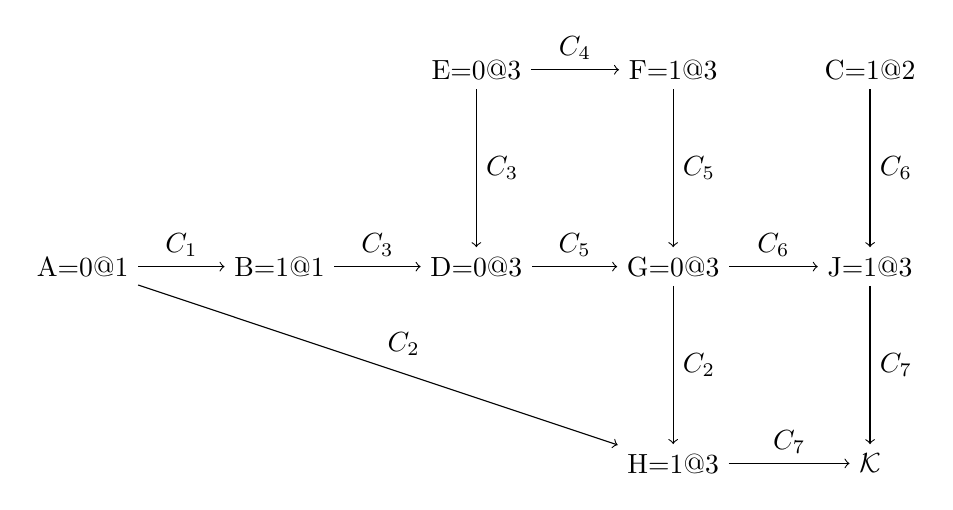
\begin{tikzpicture}[node distance=2.5cm,auto]
\node (A) {A=0@1};
\node (B) [right of=A] {B=1@1};
\node (D) [right of=B] {D=0@3};
\node (G) [right of=D] {G=0@3};
\node (H) [below of=G] {H=1@3};
\node (K) [right of=H] {$\mathcal K$};
\node (E) [above of=D] {E=0@3};
\node (F) [right of=E] {F=1@3};
\node (J) [right of=G] {J=1@3};
\node (C) [above of=J] {C=1@2};
\path[->] (G) edge node {$C_6$} (J);
\path[->] (F) edge node {$C_5$} (G);
\path[->] (C) edge node {$C_6$} (J);
\path[->] (J) edge node {$C_7$} (K);
\path[->] (E) edge node {$C_3$} (D);
\path[->] (E) edge node {$C_4$} (F);

\path[->] (A) edge node {$C_1$} (B);
\path[->] (B) edge node {$C_3$} (D);
\path[->] (D) edge node {$C_5$} (G);
\path[->] (G) edge node {$C_2$} (H);
\path[->] (H) edge node {$C_7$} (K);
\path[->] (A) edge node {$C_2$} (H);
\end{tikzpicture}%
%EndExpansion
\newline
\bigskip

  }

\item Prove that in a conflict graph the first UIP is uniquely defined, i.e.,
  prove that there is exactly one node in the graph which is a first UIP.

 %\solution{
$[p]\sigma = [x:=x+y; \text{ if } x<0 \text{ then } abort \text{ else } while \text{ } x \neq y \text{ } do \text{ }... \text{ } od]\sigma 
\hspace{0.6 cm} \sigma: x \mapsto 1, y \mapsto 1\\
= [\text{if } x<0 \text{ then } abort \text{ else } while \text{ } x \neq y \text{ } do \text{ }... \text{ } od][x:=x+y]\sigma_1
\hspace{1 cm} \sigma_1: x \mapsto [x+y]\sigma = 2\\
\text{} \hspace{12 cm} y \mapsto 1\\
= [\text{if } x<0 \text{ then } abort \text{ else } while \text{ } x \neq y \text{ } do \text{ }... \text{ } od]\sigma_1
\hspace{4 cm} \underbrace{[x<0]\sigma_1=0}_{false}\\
= [\text{while } x \neq y \text{ do } x:=x+1; y:=y+2 \text{ od}]\sigma_1
\hspace{5 cm} \underbrace{[x \neq y]\sigma_1=0}_{true}\\
= [\text{while } x \neq y \text{ do } ... \text{ od}] [x:=x+1;y=y+2]\sigma_1\\
= [\text{while } x \neq y \text{ do } ... \text{ od}] [y:=y+1] [x:=x+1]\sigma_1
\hspace{3 cm} \sigma_2: x \mapsto [x+1]\sigma_1=3\\
\text{} \hspace{11.8 cm} y \mapsto 1\\
= [\text{while } x \neq y \text{ do } ... \text{ od}] [y:=y+2]\sigma_2
\hspace{4.7 cm} \sigma_3: y \mapsto [y+2]\sigma_2=3\\
\text{} \hspace{11.8 cm} x \mapsto 3\\
= [\text{while } x \neq y \text{ do } ... \text{ od}]\sigma_3
\hspace{8 cm} \underbrace{[x \neq y]\sigma_3=0}_{false}\\
= \sigma_3$
%}

\item Let $\mathcal{C}$ be a set of clauses and $G$ a conflict graph with
  respect to $\mathcal{C}$. Prove: if a clause $C_l$ is learned following the
  first-UIP scheme, then $C_l$ is a consequence of $\mathcal{C}$.

\solution{

A formular $\upphi$ is a logical consequence of a formular $\upphi$
denoted  $\upphi \vDash \upphi'$, 

if $\Pi \vDash \upphi$ implies $\Pi \vDash \upphi'$ for all truth
assignements $\Pi$.

\textbf{Proof}:\\
$$C=\{C_1, \dots, C_n \} = \bigwedge_{i=1}^{n}C_i$$

$\overbrace{\bigwedge{Ci}}^{C} \vDash C_l$ iff

$\forall \Pi$ s.t. $\Pi \vDash \bigwedge{C_i} \Rightarrow \Pi \vDash C_l$\\

i.e. $\underbrace{\bigwedge{C_i}}_{C}$ is satisfied:

\begin{itemize}
 \item iff $\bigwedge{C_i} \land C_l$ is satisfied *\\
Equivalence rule:
* $(a \land b) \equiv \neg (a \rightarrow \neg b)$
 \item iff $\Pi \nvDash \bigwedge{\neg C_i \rightarrow C_l}, \forall\Pi$ is unsatisfied
 \item iff $\Pi \nvDash \bigwedge{C_i \land \neg C_l}$ is unsatisfied
\end{itemize}

\textbf{Substitution rule}:\\
We transform stepwise
\begin{center}
 iff $Pi \vDash \neg(\bigwedge{C_i} \rightarrow \neg C_l)$ \\
 iff $Pi \nvDash \bigwedge{C_i} \rightarrow \neg C_l$\\
 iff $Pi \nvDash \neg(\bigwedge{C_i} \land C_l)$
\end{center}

And therefor it follows:
\begin{center}
 iff $Pi \vDash \bigwedge{C_i} \land C_l$
\end{center}

learned clauses are a logical consequence of the original clauses and 
it prohibits the same conflict assignement in the further search.\\
$\Rightarrow$ learned clauses only adds redundancy to the original clauses.

\textbf{Proof}

$\Rightarrow$ if $C \vdash C_l$ then $\Rightarrow C \nvDash C_l$ the 
the deductive system is sound.\\
Suppose that $C$ is a countable set of proposition formulas i.e. 
set of clauses.

Then $C \cup \{\neg C_l\}$ is inconsistent i.e. $C \nvdash C_l$ for 
some $C_l$.

By the compactness theorem of propositional clauses there $\exists$
a finite subset $C_o \subseteq C$ s.t. $C_o \cup \{ \neg C_l\}$ is 
inconsistent i.e. has no models.\\

Then $C \vDash C_l$\\
By the existing completeness theorem of propositional calculus $C_o \vdash C_l$
Hence $C \vdash C_l$.

}

\end{enumerate}


%%%%%%%%%%%%%%%%%%%%%%%%%%%%%%%%%%%%%%%%%%%%%%%%%%%%%%%%%%%%%%%%%%%%%%%%%%%%%%

\newpage
\Aufgabe[Sparse Method \hfill \bf (1.5 points)]
Apply the Sparse Method including preprocessing on the formula $\varphi^E$
below to obtain a propositional formula.
\begin{displaymath}
  (x_1 \neq x_2 \lor x_2=x_3 ) \land \big[ (x_2 \neq x_4 \land x_3=x_4
  \land x_4=x_5)
  \lor (x_6 \neq x_5 \land x_6=x_7 \land x_7=x_3)\big]
\end{displaymath}

















  \solution{
The sparse method is a decision procedure for equality logic that computes
equi-satisfiable formulas in propositional logic.

Consider formula $\varphi ^{E}$ in equation logic:%

\begin{displaymath}
  \varphi ^{E}: (x_1 \neq x_2 \lor x_2=x_3 ) \land \big[ (x_2 \neq x_4 \land x_3=x_4
  \land x_4=x_5)
  \lor (x_6 \neq x_5 \land x_6=x_7 \land x_7=x_3)\big]
\end{displaymath}

Then the sets of equality literals and disequality literals of $\varphi ^{E}$
are:

\begin{eqnarray*}
E_{=}
&=&%
\{x_{2}=x_{3,}x_{3}=x_{4},x_{4}=x_{5},x_{6}=x_{7},x_{7}=x_{3}\}
\\
E_{\neq } &=&\{x_{1}\neq x_{2},x_{2}\neq x_{4},x_{6}\neq x_{5}\}
\end{eqnarray*}

It is very often the case, that a given equality logic formula $\varphi ^{E}$
can be simplified. Before reducing $\varphi ^{E}$ to a propositional formula 
$\varphi ^{P}$, we have to do some preprocessing for simplifying the
equality formula $\varphi ^{E}$:

\begin{enumerate}
\item Construct an equality graph $G^{E}(\varphi ^{E})=(V,E_{=},E_{\neq })$:

%\enlargethispage{100cm}
% Start of code
\begin{tikzpicture}[>=latex',line join=bevel,]
%%
\node (x2) at (101bp,99.026bp) [draw,circle] {$x_2$};
  \node (x3) at (149.22bp,182.55bp) [draw,circle] {$x_3$};
  \node (x1) at (14.5bp,99.026bp) [draw,circle] {$x_1$};
  \node (x6) at (293.9bp,99.026bp) [draw,circle] {$x_6$};
  \node (x7) at (245.67bp,182.55bp) [draw,circle] {$x_7$};
  \node (x4) at (149.22bp,15.5bp) [draw,circle] {$x_4$};
  \node (x5) at (245.67bp,15.5bp) [draw,circle] {$x_5$};
  \draw [solid] (x5) ..controls (262.06bp,43.885bp) and (277.41bp,70.467bp)  .. (x6);
  \definecolor{strokecol}{rgb}{0.0,0.0,0.0};
  \pgfsetstrokecolor{strokecol}
  \draw (276.75bp,53.203bp) node {$\neq$};
  \draw [solid] (x2) ..controls (117.39bp,70.641bp) and (132.74bp,44.059bp)  .. (x4);
  \draw (132.08bp,61.323bp) node {$\neq$};
  \draw [dashed] (x3) ..controls (149.22bp,136.43bp) and (149.22bp,61.789bp)  .. (x4);
  \draw (144.22bp,99.069bp) node {=};
  \draw [solid] (x1) ..controls (45.08bp,99.026bp) and (70.32bp,99.026bp)  .. (x2);
  \draw (57.714bp,107.03bp) node {$\neq$};
  \draw [dashed] (x2) ..controls (117.39bp,127.41bp) and (132.74bp,153.99bp)  .. (x3);
  \draw (132.08bp,136.73bp) node {=};
  \draw [dashed] (x6) ..controls (277.51bp,127.41bp) and (262.16bp,153.99bp)  .. (x7);
  \draw (262.82bp,136.73bp) node {=};
  \draw [dashed] (x4) ..controls (182bp,15.5bp) and (212.69bp,15.5bp)  .. (x5);
  \draw (197.38bp,7.5bp) node {=};
  \draw [dashed] (x7) ..controls (212.79bp,182.55bp) and (181.84bp,182.55bp)  .. (x3);
  \draw (197.36bp,174.55bp) node {=};
%
\end{tikzpicture}

The equality graph has two contradictory cycles, $%
c_{1}=(x_{2},x_{3},x_{4})$ and $%
c_{2}=(x_{3},x_{4},x_{5},x_{6},x_{7})$.

\item 
Following strictly the rules of the simplification algorithm, the algorithm
replace in this case every literal in the equality formula $\varphi ^{E}$
with \textsc{True}. In order to transform $\varphi ^{E}$ into a
propositional formula $\varphi ^{P}$, we have to make a little trick to
enforce the application of the reduction algorithm. In this case we apply
only one step of the simplification algorithm and replace all literals at
once with \textsc{True}, which are not in the cycles $c_{1}$ and $c_{2}$. So
we get:

\begin{eqnarray*}
\varphi _{1}^{E}:(\text{\textsc{True}}\vee \text{\textsc{True}})\wedge [
(x_{2}\,{\neq}\,x_{4}\wedge x_{3}\,{=}\,x_{4}\wedge x_{4}\,{=}
\,x_{5})\vee \\
(x_{5}\,{\neq}\,x_{6}\wedge x_{6}\,{=}\,x_{7}\wedge x_{3}\,{=}\,x_{7})]
\end{eqnarray*}

\begin{equation*}
\Rightarrow \;\;\varphi _{1}^{E}:(x_{2}\,{\neq}\,x_{4}\wedge x_{3}\,{=}\,x_{4}\wedge x_{4}\,{=}
\,x_{5})\vee \\
(x_{5}\,{\neq}\,x_{6}\wedge x_{6}\,{=}\,x_{7}\wedge x_{3}\,{=}\,x_{7})
\end{equation*}

Then the equality graph $G^{E}(\varphi _{1}^{E})$ looks like:

%\enlargethispage{100cm}
% Start of code
\begin{tikzpicture}[>=latex',line join=bevel,]
%%
\node (x2) at (14.5bp,90.939bp) [draw,circle] {$x_2$};
  \node (x3) at (206.21bp,14.5bp) [draw,circle] {$x_3$};
  \node (x6) at (206.21bp,167.38bp) [draw,circle] {$x_6$};
  \node (x7) at (261.75bp,90.939bp) [draw,circle] {$x_7$};
  \node (x4) at (116.35bp,43.697bp) [draw,circle] {$x_4$};
  \node (x5) at (116.35bp,138.18bp) [draw,circle] {$x_5$};
  \draw [solid] (x5) ..controls (147.27bp,148.23bp) and (175.43bp,157.38bp)  .. (x6);
  \definecolor{strokecol}{rgb}{0.0,0.0,0.0};
  \pgfsetstrokecolor{strokecol}
  \draw (158.33bp,161.8bp) node {$\neq$};
  \draw [solid] (x2) ..controls (47.335bp,75.709bp) and (83.51bp,58.93bp)  .. (x4);
  \draw (69.423bp,75.319bp) node {$\neq$};
  \draw [dashed] (x3) ..controls (175.19bp,24.579bp) and (146.8bp,33.804bp)  .. (x4);
  \draw (164.08bp,38.162bp) node {$=$};
  \draw [dashed] (x6) ..controls (225.32bp,141.07bp) and (242.72bp,117.12bp)  .. (x7);
  \draw (227.01bp,124.12bp) node {$=$};
  \draw [dashed] (x4) ..controls (116.35bp,76.211bp) and (116.35bp,105.82bp)  .. (x5);
  \draw (111.35bp,90.991bp) node {$=$};
  \draw [dashed] (x7) ..controls (242.64bp,64.635bp) and (225.23bp,40.683bp)  .. (x3);
  \draw (226.95bp,57.678bp) node {$=$};
%
\end{tikzpicture}

Now we have only the contradictory cycle $c_{2}$, and we can simplify the 
graph $G^{E}(\varphi _{1}^{E})$ once more by replacing all literals with TRUE, 
which are not in the cycle $c_{2}$. So we get a new equality graph 
$G^{E}(\varphi _{2}^{E})$:

\begin{tikzpicture}[>=latex',line join=bevel,]
%%
\node (x3) at (104.36bp,14.5bp) [draw,circle] {$x_3$};
  \node (x6) at (104.36bp,167.38bp) [draw,circle] {$x_6$};
  \node (x7) at (159.9bp,90.939bp) [draw,circle] {$x_7$};
  \node (x4) at (14.5bp,43.697bp) [draw,circle] {$x_4$};
  \node (x5) at (14.5bp,138.18bp) [draw,circle] {$x_5$};
  \draw [solid] (x5) ..controls (45.422bp,148.23bp) and (73.58bp,157.38bp)  .. (x6);
  \definecolor{strokecol}{rgb}{0.0,0.0,0.0};
  \pgfsetstrokecolor{strokecol}
  \draw (56.479bp,161.8bp) node {$\neq$};
  \draw [dashed] (x4) ..controls (14.5bp,76.211bp) and (14.5bp,105.82bp)  .. (x5);
  \draw (9.5bp,90.991bp) node {$=$};
  \draw [dashed] (x3) ..controls (73.438bp,24.547bp) and (45.28bp,33.696bp)  .. (x4);
  \draw (62.381bp,38.115bp) node {$=$};
  \draw [dashed] (x6) ..controls (123.47bp,141.07bp) and (140.87bp,117.12bp)  .. (x7);
  \draw (125.16bp,124.12bp) node {$=$};
  \draw [dashed] (x7) ..controls (140.79bp,64.635bp) and (123.38bp,40.683bp)  .. (x3);
  \draw (125.1bp,57.678bp) node {$=$};
%
\end{tikzpicture}

Recall the theorem,%
\begin{equation*}
\varphi ^{E}\text{ is satisfiable }\Leftrightarrow e(\varphi ^{E})\AND B_{t}%
\text{ is satisfiable,}
\end{equation*}

where $e(\varphi ^{E})$ denotes the \textit{propositional skeleton} of $%
\varphi ^{E}$and $B_{t}$ is a formula that describes the \textit{%
transitivity constraints} (conjunctions of implications).

So $\varphi ^{P}=e(\varphi ^{E})\AND B_{t}$ is equi-satisfiable to $\varphi
^{E}$, iff $\varphi ^{E}$ is satisfiable.

\bigskip
\item First we construct the propositional skeleton of $\varphi _{2}^{E}$ by
replacing each atom of the form $x_{i}=x_{j}$ in $\varphi _{2}^{E}$ with $%
e_{i,j}$, such that:%
\begin{equation*}
e(\varphi _{2}^{E})=(e_{3,4}\AND e_{4,5})\OR(\lnot e_{5,6}\AND e_{1,6} \AND 
e_{3,7})
\end{equation*}

\item Construct the nonpolar equality graph $G_{NP}^{E}(\varphi _{2}^{E})$:

\begin{tikzpicture}[>=latex',line join=bevel,]
%%
\node (x3) at (104.36bp,14.5bp) [draw,circle] {$x_3$};
  \node (x6) at (104.36bp,167.38bp) [draw,circle] {$x_6$};
  \node (x7) at (159.9bp,90.939bp) [draw,circle] {$x_7$};
  \node (x4) at (14.5bp,43.697bp) [draw,circle] {$x_4$};
  \node (x5) at (14.5bp,138.18bp) [draw,circle] {$x_5$};
  \draw [solid] (x5) ..controls (45.422bp,148.23bp) and (73.58bp,157.38bp)  .. (x6);
  \draw [solid] (x4) ..controls (14.5bp,76.211bp) and (14.5bp,105.82bp)  .. (x5);
  \draw [solid] (x3) ..controls (73.438bp,24.547bp) and (45.28bp,33.696bp)  .. (x4);
  \draw [solid] (x6) ..controls (123.47bp,141.07bp) and (140.87bp,117.12bp)  .. (x7);
  \draw [solid] (x7) ..controls (140.79bp,64.635bp) and (123.38bp,40.683bp)  .. (x3);
%
\end{tikzpicture}

\item Make $G_{NP}^{E}(\varphi _{2}^{E})$ chordal, using elimination
ordering $(x_{3},x_{4},x_{5},x_{6},x_{7})$:

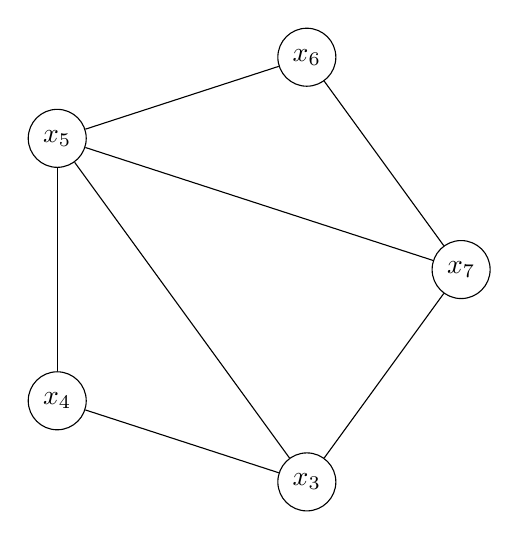
\begin{tikzpicture}[>=latex',line join=bevel,]
%%
\node (x3) at (104.36bp,14.5bp) [draw,circle] {$x_3$};
  \node (x6) at (104.36bp,167.38bp) [draw,circle] {$x_6$};
  \node (x7) at (159.9bp,90.939bp) [draw,circle] {$x_7$};
  \node (x4) at (14.5bp,43.697bp) [draw,circle] {$x_4$};
  \node (x5) at (14.5bp,138.18bp) [draw,circle] {$x_5$};
  \draw [solid] (x5) ..controls (44.939bp,148.07bp) and (73.303bp,157.29bp)  .. (x6);
  \draw [solid] (x5) ..controls (55.749bp,124.78bp) and (117.74bp,104.64bp)  .. (x7);
  \draw [solid] (x3) ..controls (73.438bp,24.547bp) and (45.28bp,33.696bp)  .. (x4);
  \draw [solid] (x3) ..controls (78.612bp,49.939bp) and (40.44bp,102.48bp)  .. (x5);
  \draw [solid] (x6) ..controls (123.47bp,141.07bp) and (140.87bp,117.12bp)  .. (x7);
  \draw [solid] (x4) ..controls (14.5bp,76.211bp) and (14.5bp,105.82bp)  .. (x5);
  \draw [solid] (x7) ..controls (140.79bp,64.635bp) and (123.38bp,40.683bp)  .. (x3);
%
\end{tikzpicture}

\item Generate the transitivity constraints in $B_{t}$ for every triangle in
the chordal graph $G_{NP}^{E}(\varphi _{2}^{E})$:

\begin{enumerate}
\item $B_{t}=$ \textsc{True}

\item For each triangle $(e_{i,j},e_{j,k},e_{i,k})$ in $G_{NP}^{E}(\varphi
_{2}^{E})$:%
\begin{eqnarray*}
B_{t}=((e_{3,4}\AND e_{4,5}\IMPL e_{3,5})\AND && \\
(e_{3,5}\AND e_{4,5}\IMPL e_{3,4})\AND && \\
(e_{3,4}\AND e_{3,5}\IMPL e_{4,5})\AND && \\
(e_{3,5}\AND e_{5,7}\IMPL e_{3,7})\AND && \\
(e_{3,7}\AND e_{3,5}\IMPL e_{5,7})\AND && \\
(e_{3,7}\AND e_{5,7}\IMPL e_{3,5})\AND && \\
(e_{5,6}\AND e_{6,7}\IMPL e_{5,7})\AND && \\
(e_{6,7}\AND e_{5,7}\IMPL e_{5,6})\AND && \\
(e_{5,6}\AND e_{5,7}\IMPL e_{6,7})) &&
\end{eqnarray*}

Hence, $\varphi ^{E}$ is satisfiable, iff $\varphi ^{P}=e(\varphi _{2}^{E})%
\AND B_{t}$ is satisfiable.
\end{enumerate}
\end{enumerate}


  }


%%%%%%%%%%%%%%%%%%%%%%%%%%%%%%%%%%%%%%%%%%%%%%%%%%%%%%%%%%%%%%%%%%%%%%%%%%%%%%

\newpage
\Aufgabe[Ackermann's Reduction \hfill \bf (1 point)]
Apply Ackermann's reduction on the following EUF-formula $\varphi$ to obtain
an EU formula:
\begin{displaymath}
  f\left(f\left(g\left(a\right),b\right),a\right) = f(g(a),b) \rightarrow \big[ f(x,y) = g(f(g(a),b)) \land
  g(f(a,y))=d \big]
\end{displaymath}

\documentclass[a4paper,parskip=half]{scrartcl}
%%%%%%%%%%%%%%%%%%%%%%%%%%%%%%%%%%%%%%%%%%%%%%%%%%%%%%%%%%%%%%%%%%%%%%%%%%%%%%%%%%%%%%%%%%%%%%%%%%%%%%%%%%%%%%%%%%%%%%%%%%%%%%%%%%%%%%%%%%%%%%%%%%%%%%%%%%%%%%%%%%%%%%%%%%%%%%%%%%%%%%%%%%%%%%%%%%%%%%%%%%%%%%%%%%%%%%%%%%%%%%%%%%%%%%%%%%%%%%%%%%%%%%%%%%%%
\usepackage{eurosym}
\usepackage[utf8]{inputenc}
\usepackage[T1]{fontenc}
\usepackage{lmodern}
\usepackage[english]{babel}
\usepackage{graphicx}
\usepackage{scrpage2}
\usepackage{ifthen}
\usepackage[ruled, boxed]{algorithm2e}
\usepackage{amsmath}
\usepackage{amsthm}
\usepackage{amssymb}
\usepackage{units}
\usepackage{enumerate}

\setcounter{MaxMatrixCols}{10}
%TCIDATA{OutputFilter=Latex.dll}
%TCIDATA{Version=5.00.0.2606}
%TCIDATA{<META NAME="SaveForMode" CONTENT="1">}
%TCIDATA{BibliographyScheme=Manual}
%TCIDATA{LastRevised=Friday, April 01, 2011 07:06:22}
%TCIDATA{<META NAME="GraphicsSave" CONTENT="32">}

\newcounter{exercise}
\setcounter{exercise}{1}
\newenvironment{exercise}[1]{\large \textsf{\textbf{Problem \arabic{exercise}}} \ifthenelse{#1>0}{(#1 points)}{} \\ \normalsize \addtocounter{exercise}{1}}{\vspace{2ex}}
\newenvironment{solution}{\large \textsf{\textbf{Solution:}} \\ \normalsize}{\vspace{2ex}}
\newenvironment{remark}{\large \textsf{\textbf{Remark}} \\ \normalsize}{\vspace{2ex}}
\newtheorem{claim}{Claim}
\newtheorem{lemma}{Lemma}
\input{tcilatex}

\begin{document}


\thispagestyle{scrheadings} ~

\subsection{solution}
\hfill \newline
At first we have to check if \textbf{Set-Partition} is a membership of NP.%
\newline
This can be shown by using a simple guess \& check procedure:\newline

Guess an arbitrary subset $S_1\subseteq S$ and verify if the sum of the
elements in $S_1$ and in $S\backslash S_1$ are equal. The summing of the
elements in the subsets takes linear time in the size of $S$.

To show NP-hardness of \textbf{Set-Partition}, we reduce \textbf{%
Subset-Sum} to \textbf{Set-Partition}.

Let $S=\{b_{1},\ldots ,b_{n}\}$ be a set of integers and an integer $t$ be a target. Let $S^{\prime }$ be an instance of 
\textbf{Set-Partition}, such that $S^{\prime }=S\cup \{c\}$ with $c=M-2\cdot
t$ and $M=\tsum\limits_{i\in S}b_{i}$.

We have to show following equation:%
\begin{equation*}
(S,t)\in 
%TCIMACRO{\TeXButton{Subset-Sum}{\mbox{\textbf{Subset-Sum}}}}%
%BeginExpansion
\mbox{\textbf{Subset-Sum}}%
%EndExpansion
\Leftrightarrow S^{\prime }\in 
%TCIMACRO{\TeXButton{Set-Partition}{\mbox{\textbf{Set-Partition}}}}%
%BeginExpansion
\mbox{\textbf{Set-Partition}}%
%EndExpansion
\end{equation*}

\begin{proof}
\hfill\newline
$\Leftarrow :$ Suppose that $S^{\prime }=\{b_{1},\ldots ,b_{n+1}\}$ is a
positive instance of \textbf{Set-Partition}. Then there exists a subset $%
S_1\subseteq S^{\prime }$,which specify the partition, such that $S_2=S^{\prime
}\backslash S_1$ and the sum of the elements in\ $S_1$ and $S_2$ are equal.

Let $S^1=\tsum\limits_{i\in S_1}b_{i}$ and $S^2=\tsum\limits_{i\in B}b_{i}$
be the sum of the elements in the subsets. Since $c=M-2\cdot t$ and $c\in
S^{\prime }$, hence $c$ is in one of the two partitions.

Without loss of generality, suppose that $c\in S_1$. Then $N=M+c=M+M-2\cdot
t=2\cdot M-2\cdot t=\tsum\limits_{i\in S^{\prime }}b_{i}$. Since $S^1=S^2
$ and $N=S^1+S^2$, it follows that $S^1=S^2=\frac{N}{2}=$ $\frac{%
2\cdot M-2\cdot t}{2}=M-t$.

Since $c\in S_1$ and $c=M-2\cdot t$, we can conclude that $S^1=t+c$. If $c$
is in the fist part of the partition, then $S_1\backslash \{c\}$ is a subset
of $S$ that sum to $t$, and if $c$ is in the second part of the partition,
then $S_2\backslash \{c\}$ is a subset of elements of $S$ that sum to $t$.
Hence, $(S,t)$ is a positive instance of \textbf{Subset-Sum}.

$\Rightarrow :$ Suppose that $(S,t)$ is a positive instance of \textbf{%
Subset-Sum}. Then there exists a subset $T\subseteq S$ such that $%
\tsum\limits_{i\in T}b_{i}=t$.

We have to show that $S^{\prime }=S\cup \{c\}$ is a positive instance of 
\textbf{Set-Partition}. Thus, we have to find two subsets of $S^{\prime }$
such that $S^1=S^2$. This can be done easily by setting $S_1=T\cup \{c\}$.
Then $S^1=t+M-2\cdot t=M-t=\frac{N}{2}$, wich is exactly the half of the
sum of elements in $S^{\prime }$, i.e. $S^1=\frac{N}{2}=S^2$. This
implies that $S^{\prime }$ is partitionable. Thus, $S^{\prime }$ is a
positive instance of \textbf{Set-Partition}.
\end{proof}

Since \textbf{Set-Partition} $\in $ NP and is NP-hard, it follows that it is
NP-complete.
\end{solution}

\begin{remark}
To see how algorithms are represented in pseudo-code see how algorithms are
described in the book \^{a}\euro \oe Introduction to Algorithms\^{a}\euro 
\"{\i}\textquestiondown 
%TCIMACRO{\U{bd} }%
%BeginExpansion
$\frac12$
%EndExpansion
by Cormen, Leiserson, Rivest, and Stein. A link to the book (that let\^{a}%
\euro \texttrademark s you browse the pages of the book) can be found on
Moodle.

Also recall the $\mathcal{O}$-notation: Let $f$ and $g$ be two functions
from the natural numbers onto the positive real numbers. If there exist
constants $c>0$ and $n_{0}\geq 0$ such that for all $n\geq n_{0}$, $f(n)\leq
c\cdot g(n)$, then we write $f(n)=\mathcal{O}(g(n))$. Let $n$ be the size of
the cost matrix of a finite game. The running time $T(n)$ of an algorithm
takes time polynomial in $n$, if there exists an integer constant $d>0$ such
that $T(n)=\mathcal{O}(n^{d})$. For more details see Chapter 3 in the above
book.
\end{remark}

\end{document}




\end{document}
